\documentclass[aspectratio=169]{beamer}

\usetheme{Boadilla}
\usefonttheme{professionalfonts}
\setbeamertemplate{navigation symbols}{}
\setbeamertemplate{itemize items}[circle]
\setbeamertemplate{enumerate items}[default]
\setbeamertemplate{headline}{}

\usepackage[utf8]{inputenc}
\usepackage[T1]{fontenc}
\usepackage{lmodern}
\usepackage{amsmath}
\usepackage{booktabs}
\usepackage{tabularx}
\usepackage{array}
\usepackage{hyperref}
\usepackage[strings]{underscore}
\usepackage{listings}
\usepackage{tikz}
\usetikzlibrary{arrows.meta,positioning,fit,calc,shapes.geometric}
\usepackage{xcolor}

\definecolor{courseblue}{HTML}{12355B}
\definecolor{coursegold}{HTML}{C98A2E}
\definecolor{courseice}{HTML}{EEF3F8}
\definecolor{coursegreen}{HTML}{2F6B4F}
\definecolor{coursegray}{HTML}{4B5563}
\definecolor{codebg}{HTML}{F7F9FC}
\definecolor{codecomment}{HTML}{5E6C84}
\definecolor{codestring}{HTML}{0B6E4F}

\setbeamercolor{palette primary}{bg=courseblue,fg=white}
\setbeamercolor{palette secondary}{bg=coursegold,fg=white}
\setbeamercolor{palette tertiary}{bg=courseblue,fg=white}
\setbeamercolor{palette quaternary}{bg=coursegold,fg=white}
\setbeamercolor{structure}{fg=courseblue}
\setbeamercolor{frametitle}{bg=courseice,fg=courseblue}
\setbeamercolor{title}{fg=courseblue}
\setbeamercolor{block title}{bg=courseblue,fg=white}
\setbeamercolor{block body}{bg=courseice,fg=black}
\setbeamercolor{normal text}{fg=black,bg=white}
\setbeamercolor{alerted text}{fg=coursegold}

\setbeamerfont{footline}{size=\scriptsize}

\setbeamertemplate{footline}{
  \leavevmode
  \hbox{
    \begin{beamercolorbox}[wd=.33\paperwidth,ht=2.8ex,dp=1.2ex,leftskip=0.8em]{palette primary}%
      University of Trieste
    \end{beamercolorbox}%
    \begin{beamercolorbox}[wd=.49\paperwidth,ht=2.8ex,dp=1.2ex,center]{palette tertiary}%
      \coursename{} \textbar{} \coursecode
    \end{beamercolorbox}%
    \begin{beamercolorbox}[wd=.18\paperwidth,ht=2.8ex,dp=1.2ex,rightskip=0.8em plus1fil]{palette secondary}%
      \insertframenumber{} / \inserttotalframenumber
    \end{beamercolorbox}%
  }
}

\hypersetup{
  colorlinks=true,
  linkcolor=courseblue,
  urlcolor=coursegreen
}

\lstdefinestyle{coursepython}{
  language=Python,
  basicstyle=\ttfamily\footnotesize,
  keywordstyle=\color{courseblue}\bfseries,
  commentstyle=\color{codecomment}\itshape,
  stringstyle=\color{codestring},
  showstringspaces=false,
  columns=fullflexible,
  keepspaces=true,
  frame=single,
  framerule=0.6pt,
  rulecolor=\color{courseblue},
  backgroundcolor=\color{codebg},
  xleftmargin=0.4em,
  xrightmargin=0.4em,
  aboveskip=0.4em,
  belowskip=0.2em
}

\newcommand{\coursename}{Data-driven Systems Engineering}
\newcommand{\coursecode}{440MI / 305SM}
\newcommand{\coursefooter}{}

\newcommand{\learninggoals}[1]{
  \begin{block}{Learning goals}
  #1
  \end{block}
}

\newcommand{\repoactivity}[1]{
  \begin{block}{Repo activity}
  #1
  \end{block}
}

\newcommand{\readinglist}[1]{
  \begin{block}{Papers and materials}
  {\footnotesize #1}
  \end{block}
}

\newcommand{\coursecontextframe}[5]{
  \begin{frame}{Course Map and Running Cases}
  \centering
  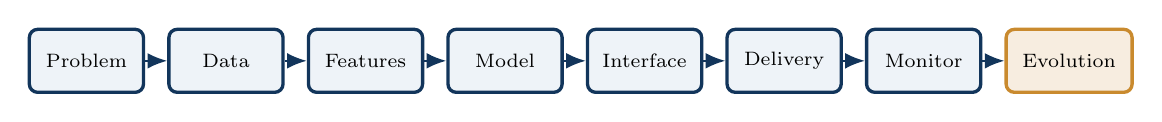
\begin{tikzpicture}[node distance=0.28cm]
  \node[flowbox, minimum width=1.45cm, minimum height=0.8cm] (problem) {\scriptsize Problem};
  \node[flowbox, minimum width=1.45cm, minimum height=0.8cm, right=of problem] (data) {\scriptsize Data};
  \node[flowbox, minimum width=1.45cm, minimum height=0.8cm, right=of data] (features) {\scriptsize Features};
  \node[flowbox, minimum width=1.45cm, minimum height=0.8cm, right=of features] (model) {\scriptsize Model};
  \node[flowbox, minimum width=1.45cm, minimum height=0.8cm, right=of model] (interface) {\scriptsize Interface};
  \node[flowbox, minimum width=1.45cm, minimum height=0.8cm, right=of interface] (delivery) {\scriptsize Delivery};
  \node[flowbox, minimum width=1.45cm, minimum height=0.8cm, right=of delivery] (monitor) {\scriptsize Monitor};
  \node[accentbox, minimum width=1.6cm, minimum height=0.8cm, right=of monitor] (evolution) {\scriptsize Evolution};
  \foreach \a/\b in {problem/data,data/features,features/model,model/interface,interface/delivery,delivery/monitor,monitor/evolution} {
    \draw[arrow] (\a) -- (\b);
  }
  \end{tikzpicture}

  \vspace{0.5em}
  \begin{block}{Today in the course}
  \textbf{Focus:} #1

  \textbf{Bridge:} #2
  \end{block}

  \begin{columns}[T]
  \column{0.48\textwidth}
  \begin{block}{Fraud case}
  {\footnotesize #3}
  \end{block}
  \column{0.48\textwidth}
  \begin{block}{Pasteurization case}
  {\footnotesize #4}
  \end{block}
  \end{columns}

  \vspace{0.3em}
  {\footnotesize \textbf{Course thread:} #5}
  \coursefooter
  \end{frame}
}

\newcommand{\classclosingframe}[4]{
  \begin{frame}{From This Class to the Next}
  \begin{block}{What stays with us}
  #1
  \end{block}

  \begin{columns}[T]
  \column{0.48\textwidth}
  \begin{block}{Project use}
  {\footnotesize #2}
  \end{block}
  \column{0.48\textwidth}
  \begin{block}{Next connection}
  {\footnotesize #3}
  \end{block}
  \end{columns}

  \vspace{0.3em}
  {\footnotesize \textbf{Course thread:} #4}
  \coursefooter
  \end{frame}
}

\tikzset{
  flowbox/.style={
    rounded corners=3pt,
    draw=courseblue,
    fill=courseice,
    very thick,
    minimum width=2.2cm,
    minimum height=0.9cm,
    align=center,
    font=\small
  },
  accentbox/.style={
    rounded corners=3pt,
    draw=coursegold,
    fill=coursegold!15,
    very thick,
    minimum width=2.2cm,
    minimum height=0.9cm,
    align=center,
    font=\small
  },
  arrow/.style={
    -{Latex[length=2.5mm,width=2mm]},
    thick,
    draw=courseblue
  }
}


\title{Class 36: Proposal Presentations, Part 2}
\subtitle{Session 36 of 36 -- Second Half, and Closing the Course}
\author{\coursename}
\date{18 December}

\begin{document}

\frame{\titlepage \coursefooter}

\begin{frame}{Agenda}
\begin{itemize}
\item Logistics for the second half
\item Quick recap of the rubric
\item Closing the course: from Class 1 to Class 36
\item Thanks, and what comes next
\end{itemize}
\coursefooter
\end{frame}

\begin{frame}{Same rubric, remaining teams, then we close}
\learninggoals{
\begin{itemize}
\item Continue today's presentations under the same format and rubric as this morning.
\item Give and receive feedback consistently across both halves of the day.
\item Connect today's work back to the full 36-session arc of the course.
\end{itemize}
}
\coursefooter
\end{frame}

\coursecontextframe
{Continuing today's presentations and closing the 36-session course.}
{The rubric and format from Class 35 carry over unchanged; this is the same session split across the day for scheduling, not a new topic.}
{Fraud-pattern projects and their variations have anchored one half of this course's running examples since Class 1.}
{Pasteurization-pattern projects and their variations have anchored the other half in the same way.}
{The Problem, Data, Features, Model, Interface, Delivery, Monitor, Evolution map used since the first class map is the same map every team's project should now fit into.}

\begin{frame}{Logistics for the second half}
\begin{itemize}
\item Same format as this morning: 10 minutes presenting, 5 minutes of questions per team.
\item Remaining teams present in the posted order; be ready 5 minutes before your slot.
\item The same rubric from Class 35 applies without change.
\item Written peer feedback is still expected from every non-presenting team.
\end{itemize}
\coursefooter
\end{frame}

\begin{frame}{Rubric, quick recap}
\begin{tabularx}{\textwidth}{>{\bfseries}l X}
Criterion & What reviewers look for \\
\toprule
Problem clarity & A specific problem and user, not a vague topic area. \\
Feasibility & Scope matches the time and data actually available. \\
Lifecycle coverage & Requirements, delivery, and monitoring are at least sketched. \\
Risk awareness & Real risks are named, with a plausible response. \\
Communication & The team can explain choices and answer questions clearly. \\
\bottomrule
\end{tabularx}
\coursefooter
\end{frame}

\begin{frame}{Closing the course: the full arc}
\centering
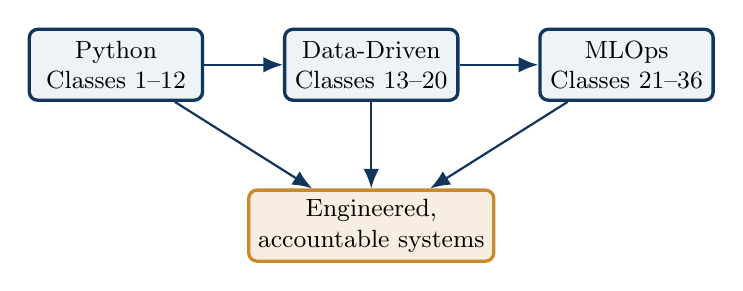
\begin{tikzpicture}[node distance=0.9cm and 1cm]
\node[flowbox] (py) {Python\\Classes 1--12};
\node[flowbox, right=of py] (dd) {Data-Driven\\Classes 13--20};
\node[flowbox, right=of dd] (ml) {MLOps\\Classes 21--36};
\node[accentbox, below=1.1cm of dd] (systems) {Engineered,\\accountable systems};
\draw[arrow] (py) -- (dd);
\draw[arrow] (dd) -- (ml);
\draw[arrow] (py) -- (systems);
\draw[arrow] (dd) -- (systems);
\draw[arrow] (ml) -- (systems);
\end{tikzpicture}
\vspace{0.4em}
\begin{itemize}
\item Thirty-six sessions, two running cases, and one repeated question: is this a good model, or a good system?
\end{itemize}
\coursefooter
\end{frame}

\begin{frame}{What should stay with you}
\begin{itemize}
\item Python and modeling skills are necessary but not sufficient on their own.
\item Requirements, process, and delivery discipline are what let a model become a system others can trust.
\item Monitoring and scaling are not afterthoughts; they are where systems actually get tested, in production, over time.
\item The fraud and pasteurization cases were vehicles for these ideas, not the point of the course.
\end{itemize}
\coursefooter
\end{frame}

\begin{frame}{Discussion prompt}
\begin{block}{Question}
What is the one habit from this course you intend to keep using after today, on a project this course never assigned?
\end{block}
\begin{itemize}
\item This closes the course on transfer, not recall.
\item There is no wrong answer; the point is naming something specific enough to actually keep doing.
\end{itemize}
\coursefooter
\end{frame}

\begin{frame}{Thanks}
\begin{itemize}
\item Thank you for thirty-six sessions of work, questions, and projects.
\item The two running cases, fraud detection and pasteurization monitoring, were teaching tools; your own projects are the real outcome.
\item Keep the habits: write the requirement down, test before you trust it, watch it after you ship it.
\end{itemize}
\coursefooter
\end{frame}

\begin{frame}{Papers and materials}
\readinglist{
For continued reading beyond this course:\
\href{https://www.oreilly.com/library/view/practical-mlops/9781098103002/}{Practical MLOps};\
\href{https://neptune.ai/blog/mlops-best-practices}{MLOps best practices overview};\
\href{https://itrevolution.com/product/accelerate/}{Forsgren, Humble, Kim, Accelerate}.
}
\coursefooter
\end{frame}

\classclosingframe
{\begin{itemize}
\item A finished proposal defense is evidence of the full lifecycle habit this course tried to build.
\item Software engineering, data-driven methods, and MLOps are one integrated way of building systems, not three separate topics.
\item The systems view from the very first class map is the same view every team just defended.
\end{itemize}}
{Your presented plan, and the feedback you received today, are what carry directly into building and delivering the actual project.}
{There is no Class 37; what comes next is project execution, delivery, and the final evaluation of each team's system.}
{The course closes with the same question it opened with: not just whether the model works, but whether the system around it can be trusted.}

\end{document}
